\chapter{Diagrammes}
\label{s:Diagrammes}




\section{Diagramme de classe}

Puisque la taille du diagramme de classe est tr�s grande, celui-ci peut �tre retrouv� � l'int�rieur du dossier /fig inclut avec la remise. Une br�ve description du flot d'ex�cution de la routine suivra afin de mieux comprendre l'utilit� des classes principales.
\medbreak

Du c�t� de la station de base, l'interface est d'abord initialis�e par le main. Ensuite, les boutons peuvent �tre utilis�s afin de d�marrer une certaine routine en initialisant la classe StationBase avec la table de jeux utilis�e et la routine voulue. Ce thread est le contr�leur de la station et est celui qui initialise par la suite les threads suivants: 
\begin{enumerate}
\item \textbf{StationServeur :} Initialise une connexion TCP avec le robot (avec TCPServeur). Il est en charge d'envoyer et de traiter toute communication entre la station de base et le robot. La communication est effectu�e sous forme d'envoie de fichier JSON qui sont cr��s par la classe RequeteJSON.
\item \textbf{FeedVideoStation :} Ce thread ne fait que lire les images de la cam�ra world afin qu'elles soient analys�es par la suite.
\item \textbf{AnalyseImageWorld :} Rep�re les iles, les tr�sors et le robot avec l'aide de plusieurs classes de d�tection. Pour la d�tection des �l�ments, les intervalles de couleur sont celles correspondantes � la table actuelle d�finit lors de l'initialisation de la station de base. Une fois trouv�s, tous les �l�ments cartographiques sont ajout� � la classe Carte.
\item \textbf{ImageVirtuelle :} Ce thread est en charge de dessiner sur l'image obtenue, afin de l'afficher dans l'interface. Les informations telles que la trajectoire pr�vue, la position r�elle du robot et les autres �l�ments cartographiques d�tect�s. Cette classe repr�sente donc tout simplement la carte virtuelle.
\end{enumerate}
Suite � l'initialisation de StationBase, Interface initialise un dernier thread (AfficherImageVirtuelle). Celui-ci ne fait que mettre � jour le feed vid�o (ImageVirtuelle) dans l'interface.  
\medbreak
D�s le d�but de l'ex�cution, la classe StationBase initialise la classe Trajectoire avec GrilleCellule. Celle-ci repr�sente la matrice de position o� le robot peut �tre positionn�. Lors de la demande d'un trajet, Trajectoire appelle AlgorithmeTrajectoire avec la grille de cellule. Cette classe trouvera la trajectoire demand�e selon le contenu des cellules. 
\medbreak
Finalement, la classe RedirigeurTexte sert tout simplement � rediriger les impressions consoles dans la boite de texte de l'interface.\bigbreak
Du cot� du robot, le contr�leur est la classe Robot. La communication se d�roule comme avec la station de base avec les classes (RequeteJSON, RobotClient, TCPClient). La classe UARTDriver est utilis�e pour envoyer des commandes par UART, tandis que la classe LectureUART est utilis�e pour lire et traiter les donn�es envoy�es par le UART.
\medbreak
Lorsque le robot entre en phase d'alignement, il se sert de AnalyseImageEmbarquee et de la classe de d�tection correspondante afin de trouver les ajustements requis. Les ajustements sont ensuite transmis au robot et sont envoy�es au UART afin de terminer la phase d'alignement.
\medbreak
La classe RobotService est utilis�e pour effectuer du traitement d'information. Elle est utilis�e pour effectuer la requ�te au serveur des iles, gr�ce au code Manchester pr�alablement d�cod�. Ensuite, elle traite la r�ponse pour obtenir l'indice sur l'ile cible.
\bigbreak
Finalement, la classe ConfigPath est utilis�e afin de transformer les adresses locales en adresses absolues. 

\section{Diagrammes de s�quence}

Les diagrammes \ref{f:ds1} � \ref{f:ds5} repr�sentent quelques s�quences d'ex�cutions importantes de notre syst�me.

\begin{figure}[htp]
   \centering
   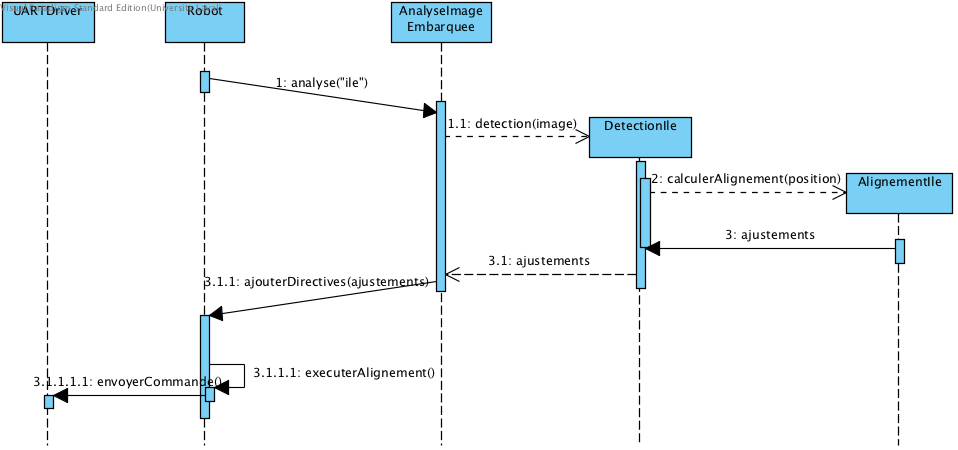
\includegraphics[width=1\textwidth]{fig/Alignement.png}
   \caption{Alignement}
   \label{f:ds1}
\end{figure}

\begin{figure}[htp]
   \centering
   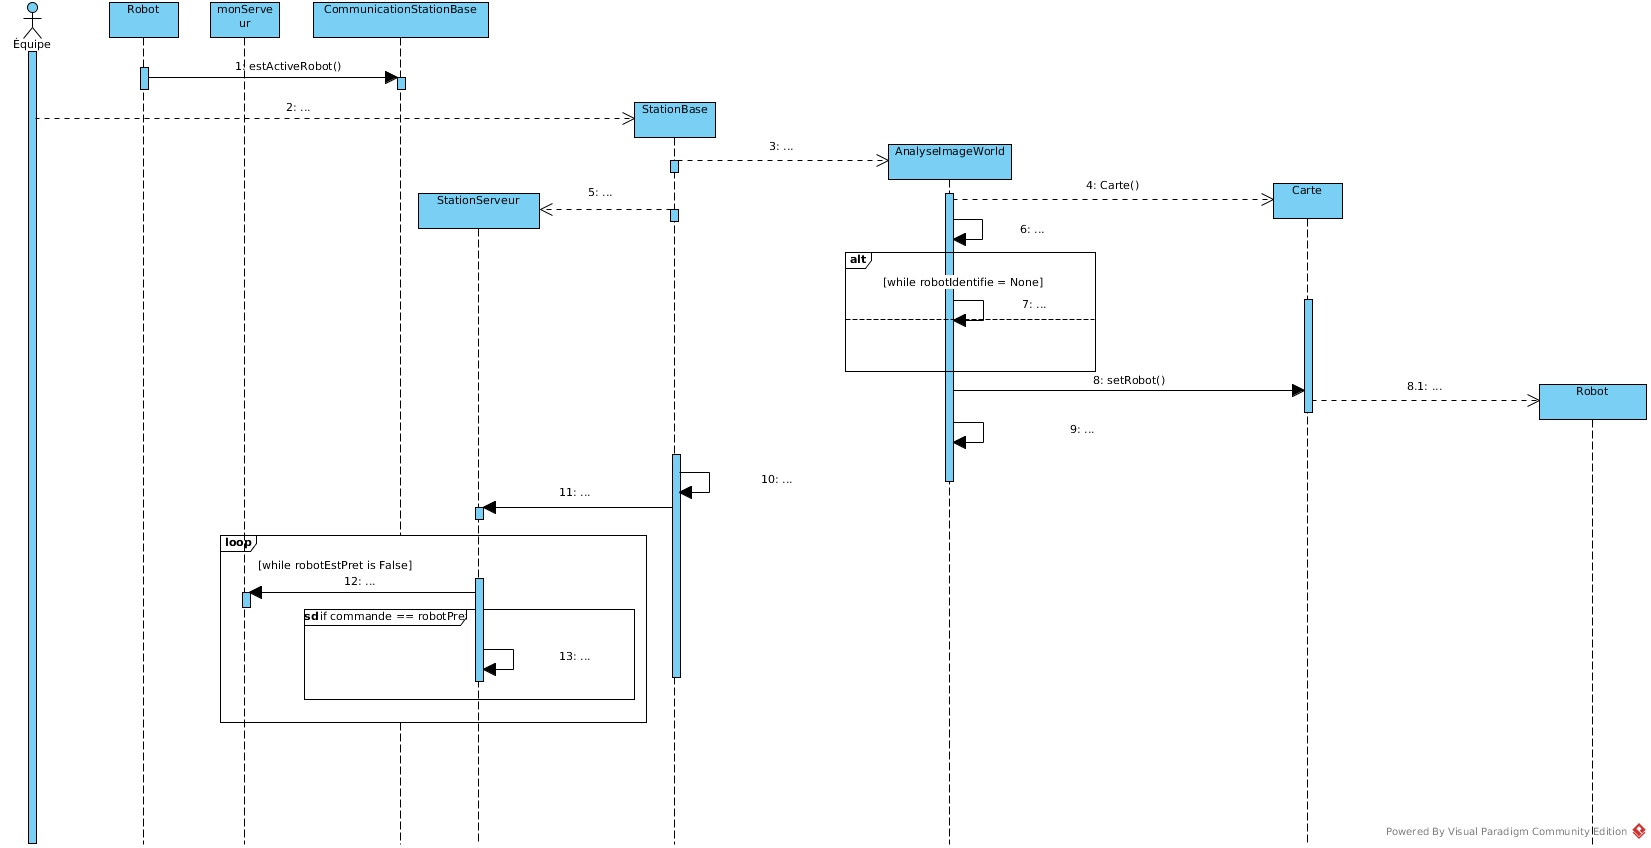
\includegraphics[width=1\textwidth]{fig/DemarageRobot.jpg}
   \caption{D�marrage du robot}
   \label{f:ds2}
\end{figure}

\begin{figure}[htp]
   \centering
   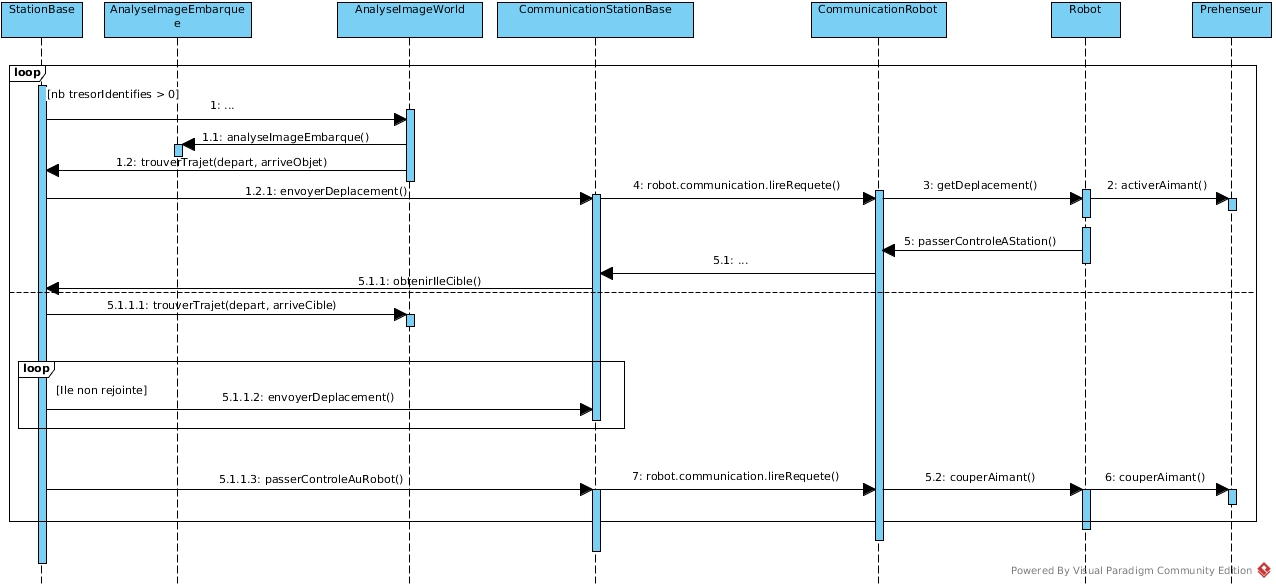
\includegraphics[width=1\textwidth]{fig/DeplaceTresor.jpg}
   \caption{D�placement du tr�sor}
   \label{f:ds3}
\end{figure}

\begin{figure}[htp]
   \centering
   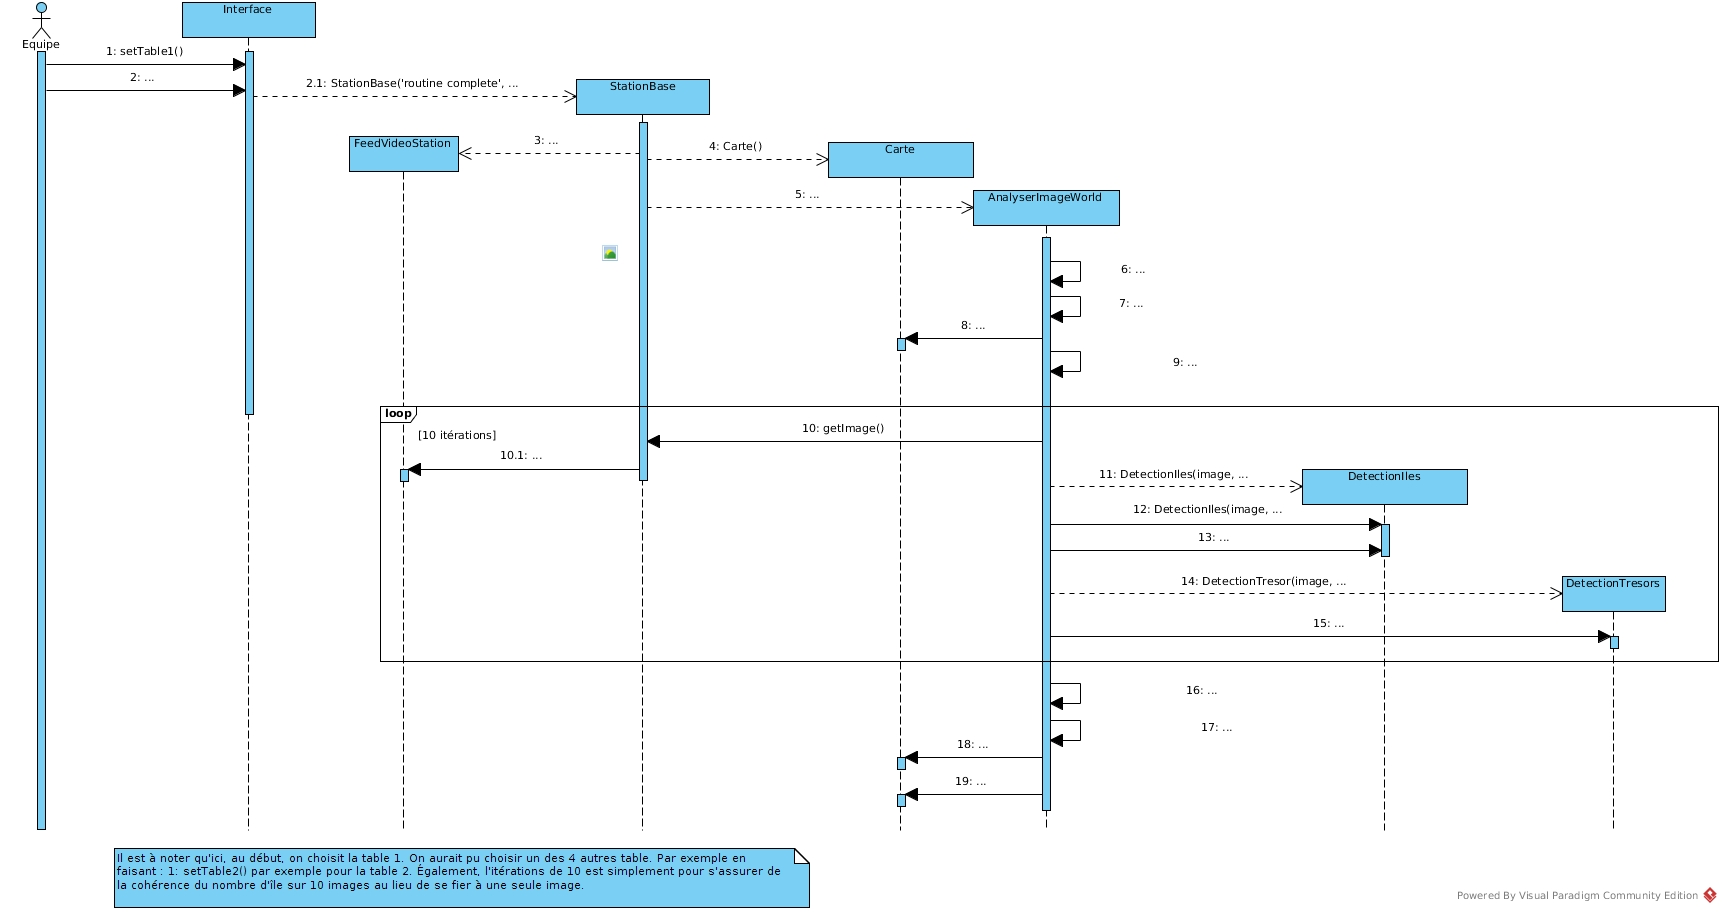
\includegraphics[width=1\textwidth]{fig/InitialiserCarte.jpg}
   \caption{Initialisation de la carte}
   \label{f:ds4}
\end{figure}

\begin{figure}[htp]
   \centering
   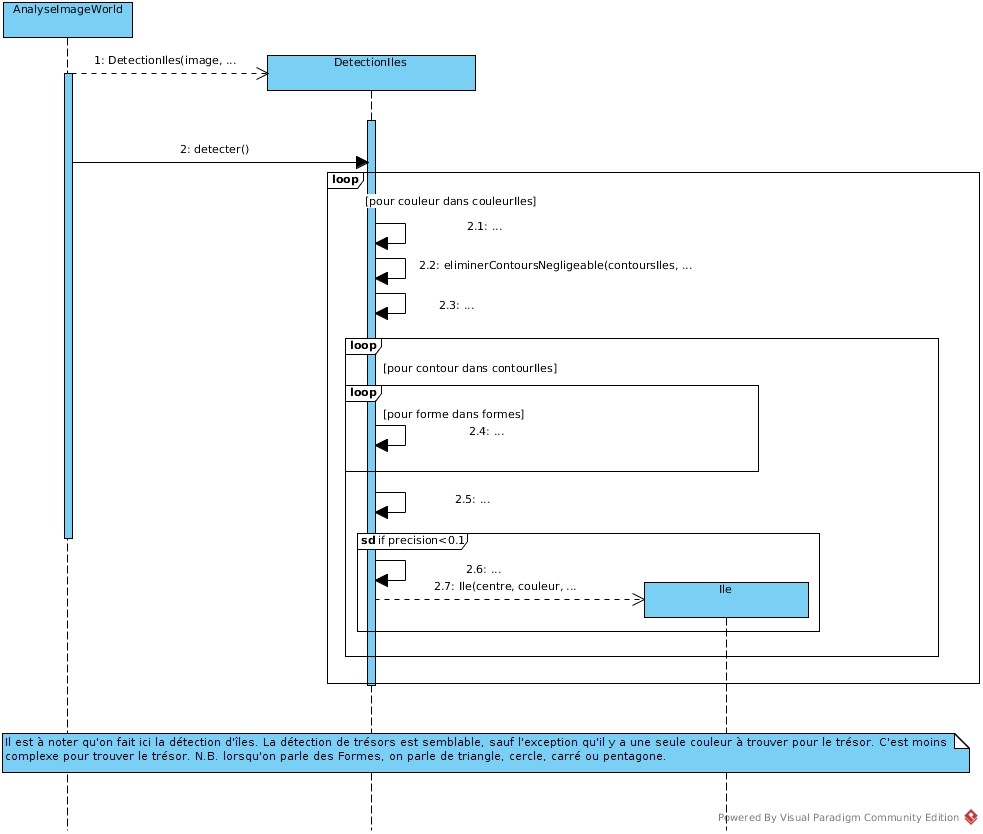
\includegraphics[width=1\textwidth]{fig/trouverIlesOuTresor.jpg}
   \caption{Trouver les �les et les tr�sors}
   \label{f:ds5}
\end{figure}

%\begin{figure}[htp]
%   \centering
%   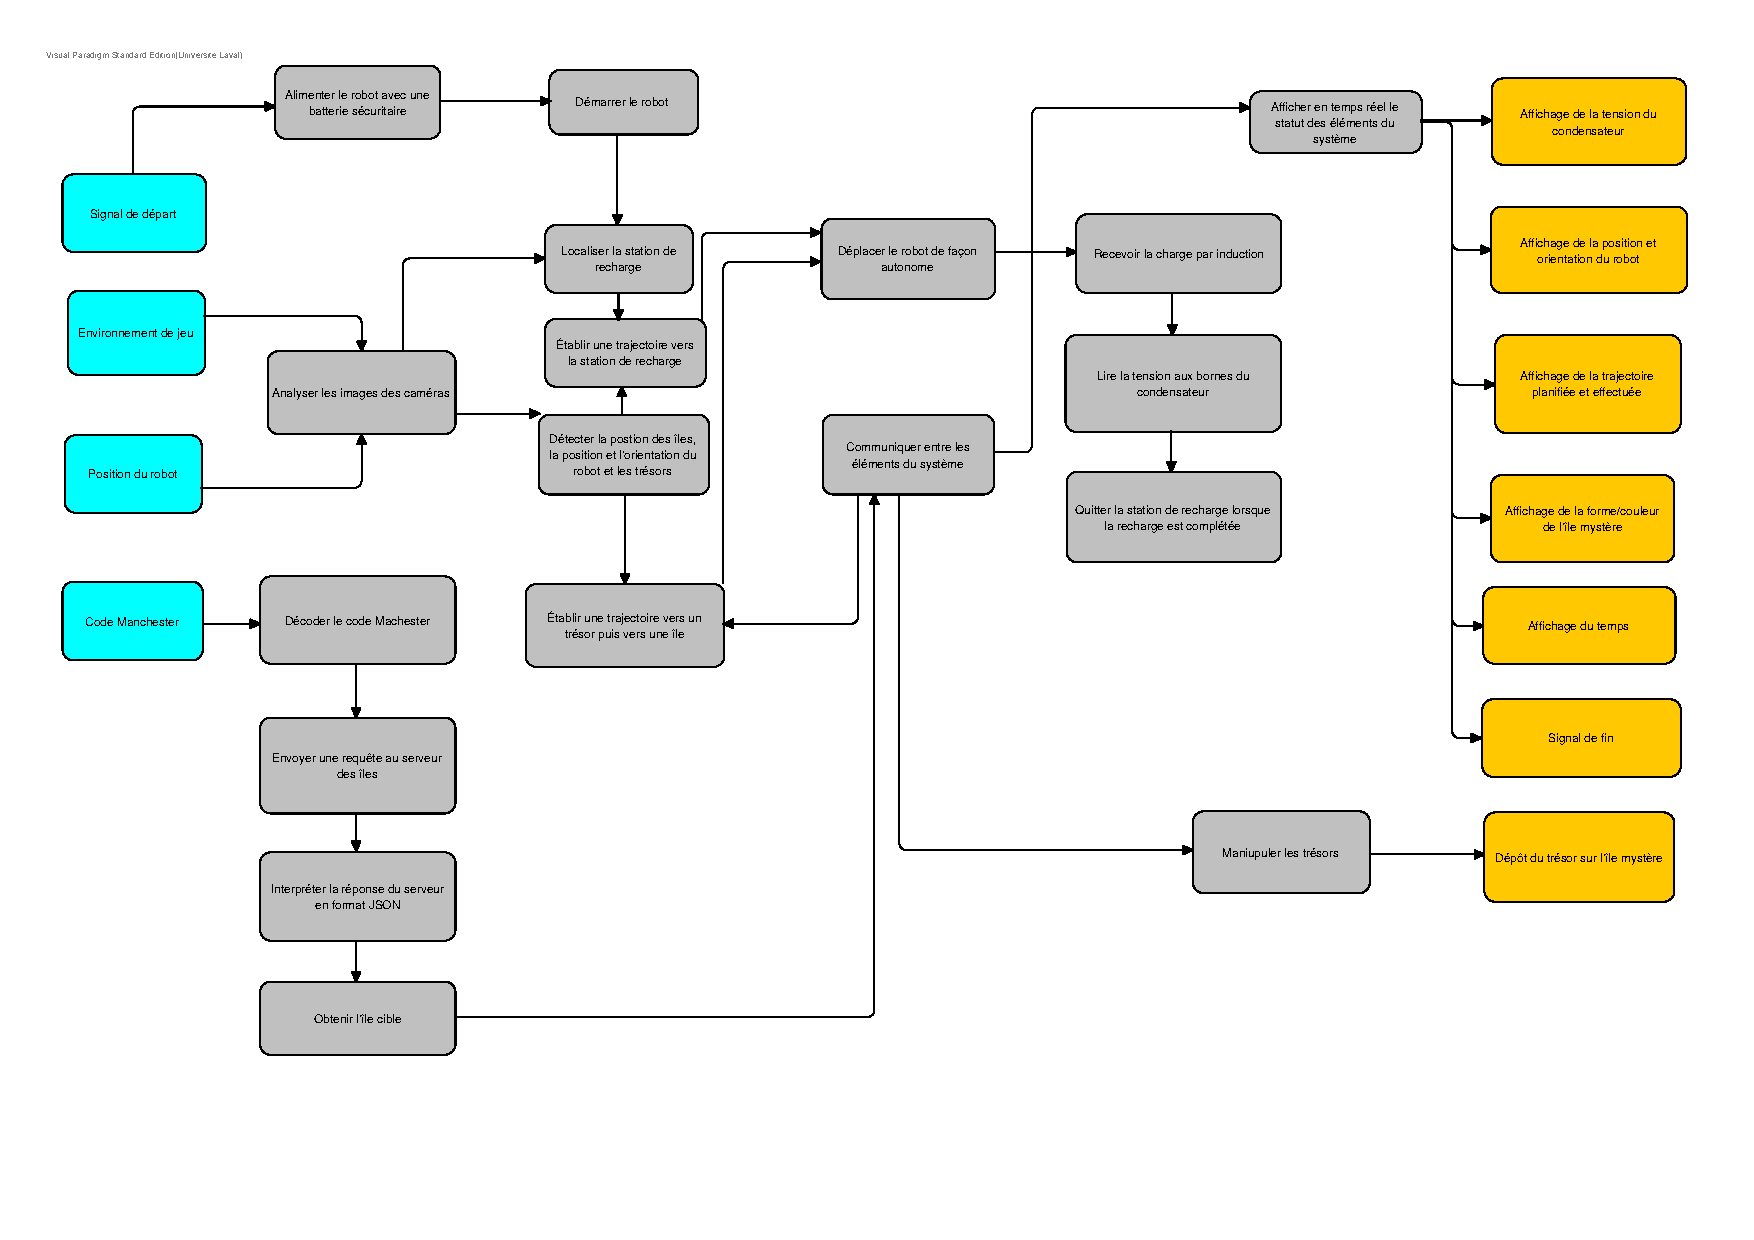
\includegraphics[width=1\textwidth]{pdf/DiagrammeFonctionnalites.pdf}
%   \caption{Diagramme des fonctionnalit�s}
%   \label{f:diagramme_fonctionnalites}
%\end{figure}


%\section{Diagramme physique}
%\label{s:diagramme_physique}

%\begin{figure}[htp]
%   \centering
%   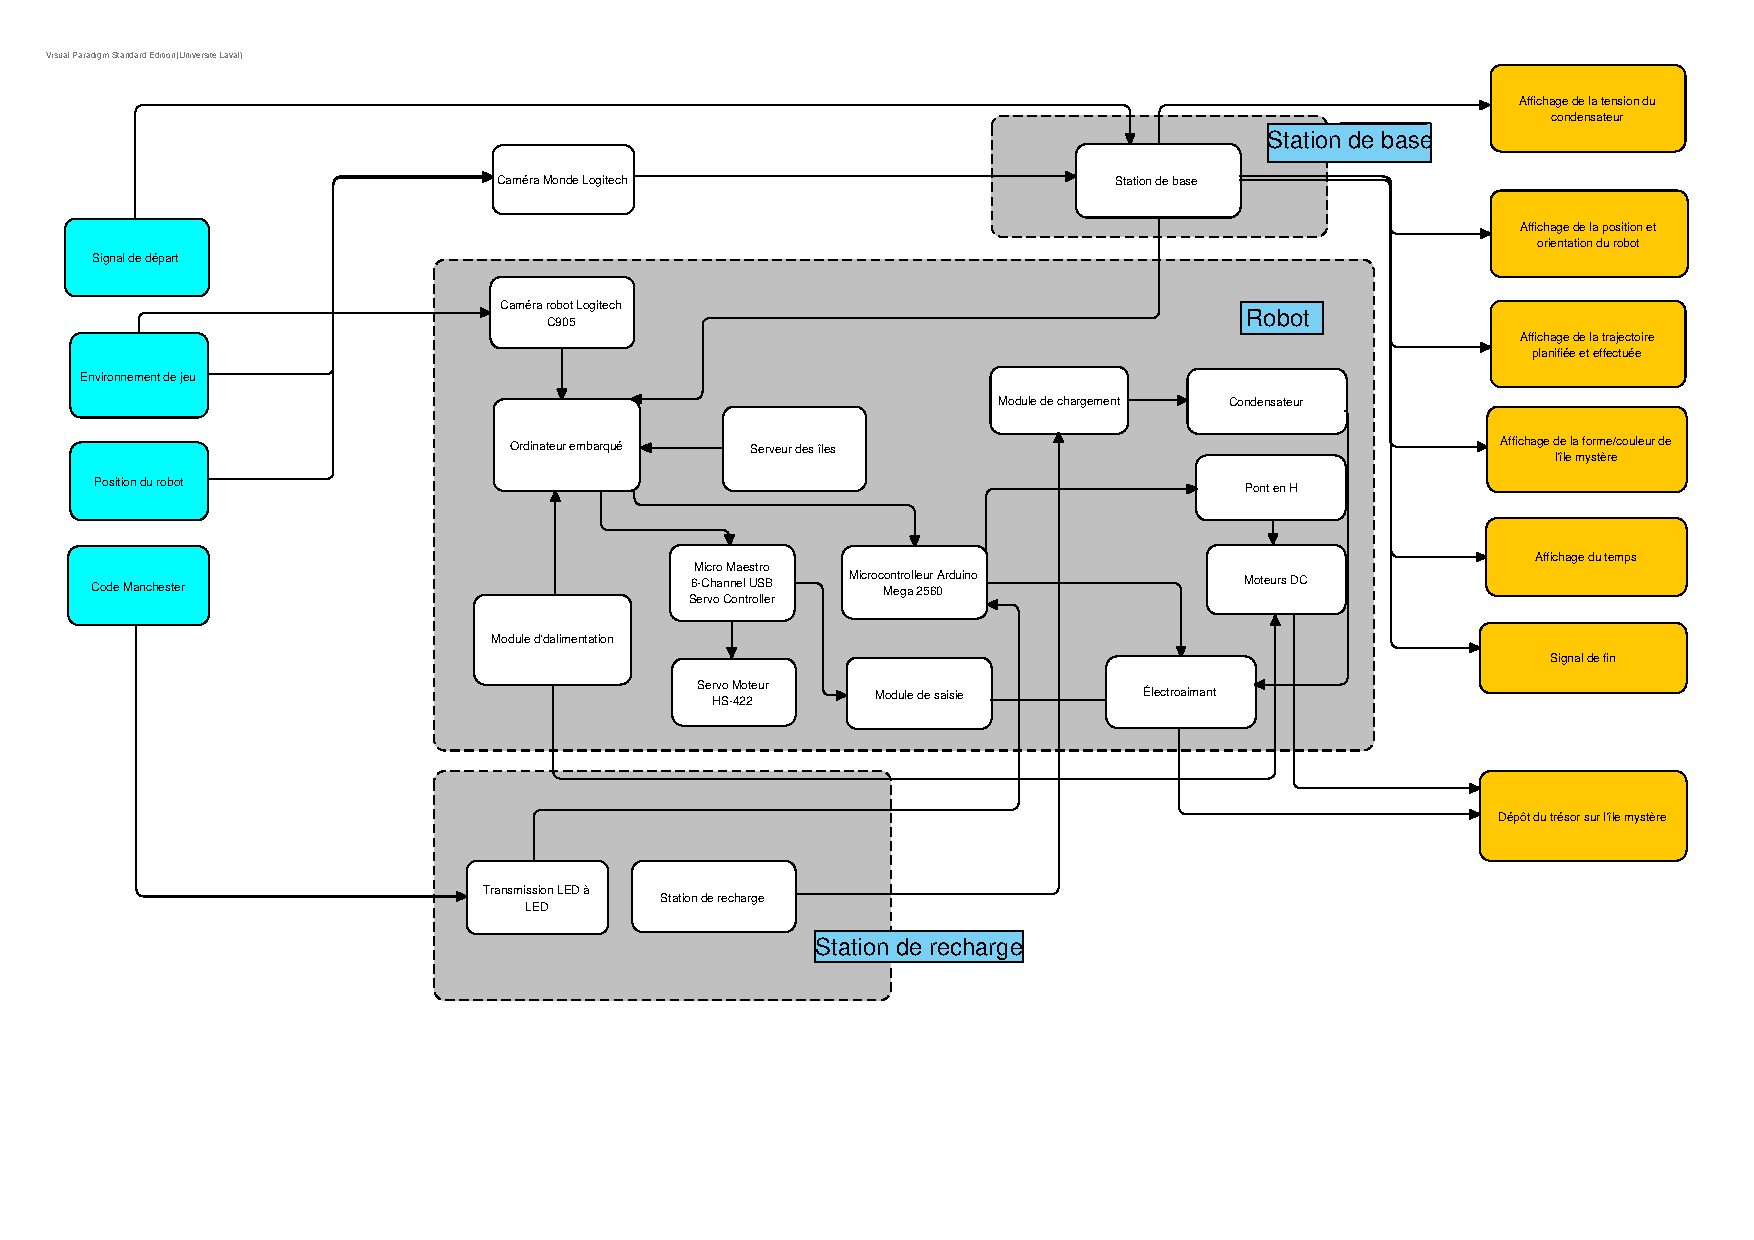
\includegraphics[width=1\textwidth]{pdf/DiagrammePhysique.pdf}
%   \caption{Diagramme physique}
%   \label{f:diagramme_physique}
%\end{figure}

%\section{Diagramme de s�quences}
%\label{s:diagramme_sequence}

%Les figures \ref{f:diagramme_sequence1} � \ref{f:diagramme_sequence4} correspondent aux diagrammes de s�quences.

%\begin{figure}[htp]
%   \centering
%   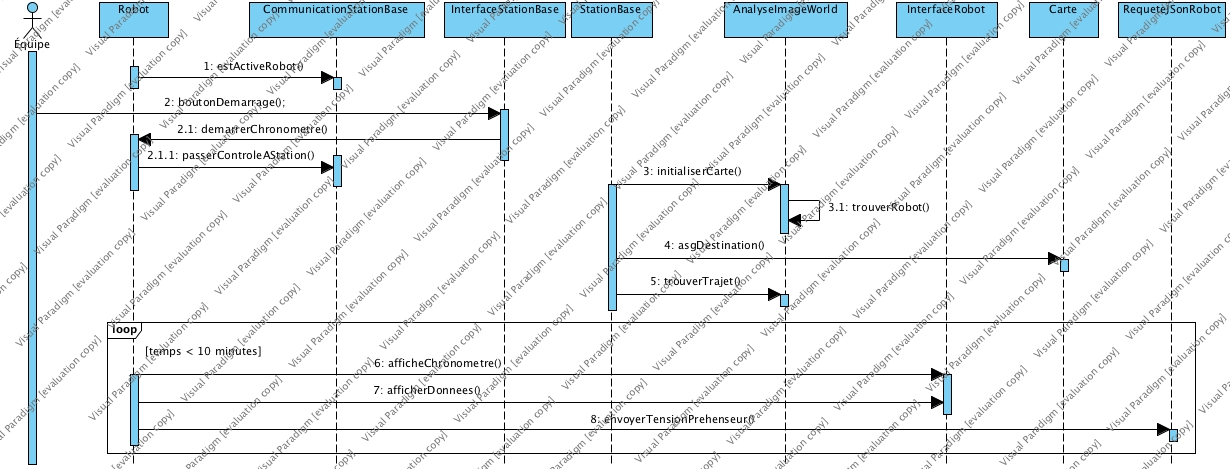
\includegraphics[width=1\textwidth]{fig/demarageRobot.jpg}
%   \caption{Diagramme de s�quences: d�marage du robot}
%   \label{f:diagramme_sequence1}
%\end{figure}

%\begin{figure}[htp]
%   \centering
%   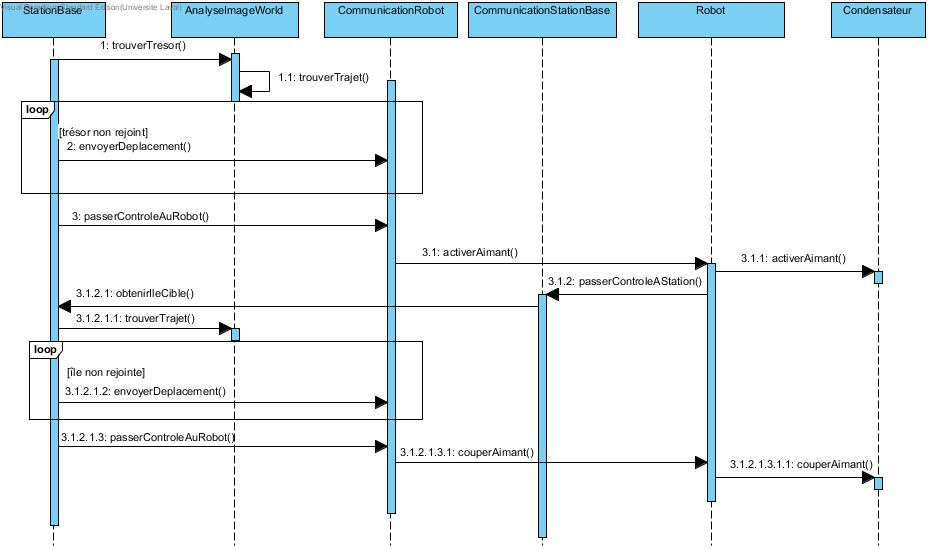
\includegraphics[width=1\textwidth]{fig/deplaceTresor.jpg}
%   \caption{Diagramme de s�quences: Deplacement du tr�sor}
%   \label{f:diagramme_sequence2}
%\end{figure}

%\begin{figure}[htp]
%   \centering
%   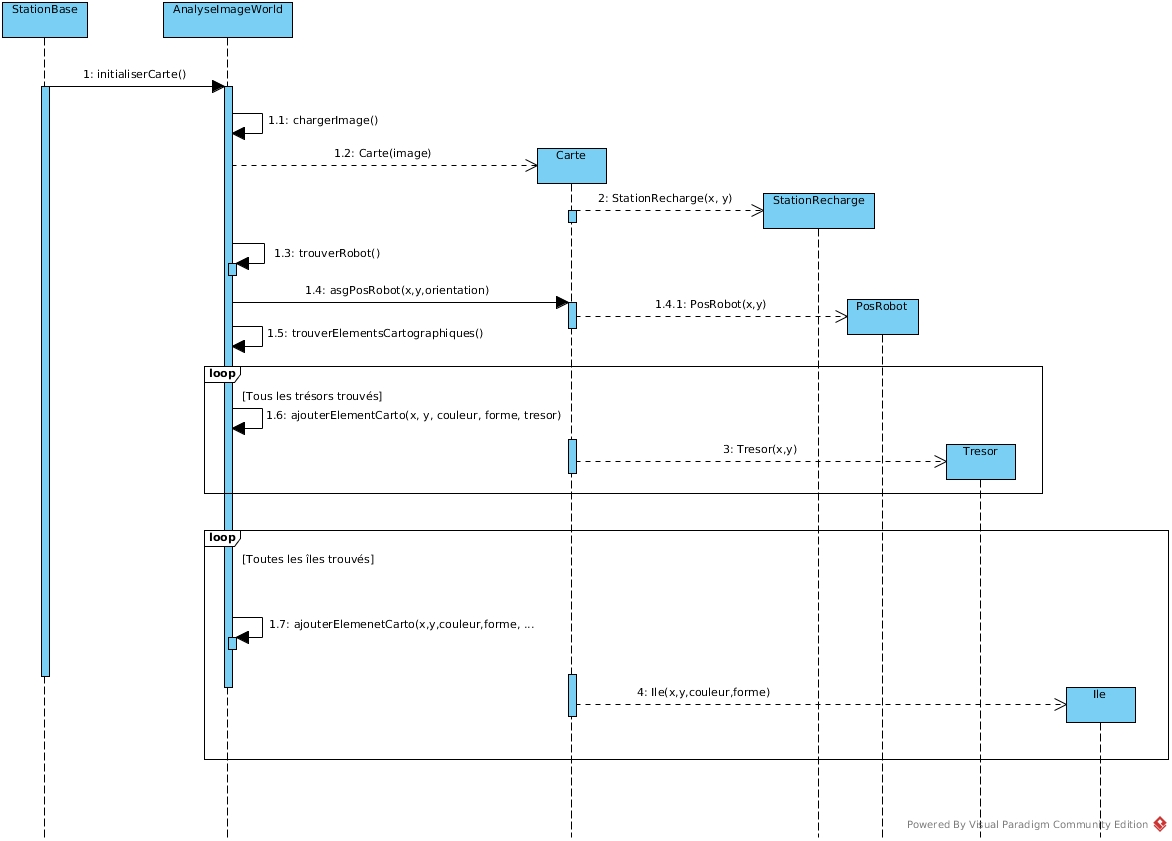
\includegraphics[width=1\textwidth]{fig/initCarte.jpg}
%   \caption{Diagramme de s�quences: initialisation de la carte}
%   \label{f:diagramme_sequence3}
%\end{figure}

%\begin{figure}[htp]
%   \centering
%   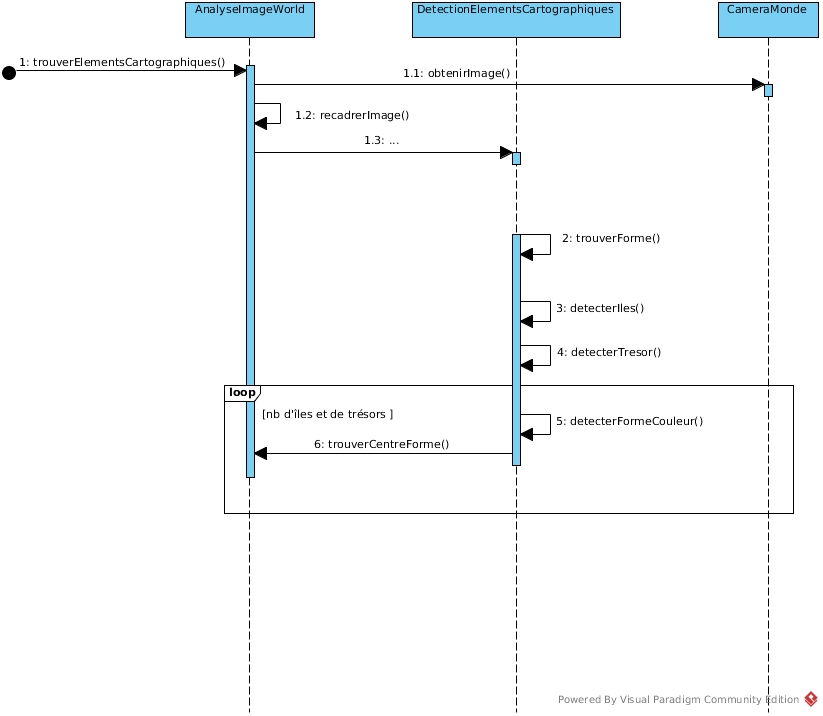
\includegraphics[width=1\textwidth]{fig/trouverIleOuTresor.jpg}
%   \caption{Diagramme de s�quences: trouver les �les et tr�sors}
%   \label{f:diagramme_sequence4}
%\end{figure}
